\section{Generatory liczb równomiernych}
	\begin{frame}{Generatory liczb równomiernych}


	\textbf{Ogólnie}
	\[
	x_{n+1}=f(\underbrace{x_{n},x_{n-1},\ldots,x_{n-k+1}}_{k \:stalych\: poczatkowych}) (mod\ \ M)
	\]
	Założenie:
	$$
	Z_{M}=\{0,\ 1,\ .\ .\ .\ ,\ M-1\}
	$$
	$$
	\text{Dziedzina } D(f)=Z_{M}^{\otimes{k}}
	$$
	$$
	\text{Przeciwdziedzina } D^{-1}(f)=Z_{M}
	$$
	Takie generatory są {\it okresowymi}:\\

	\begin{center}
	$\exists N, r:\forall n\geq N$   $x_{n}=x_{n+jr}$ , $j=1, 2, . $
	\end{center}
	$r$ - okres ciągu\\
	$\underbrace{x_{0},...,\textrm{\colorbox{red}{$x_{N}$}}, \textrm{\colorbox{blue}{$x_{N+1}$}}, ..., x_{N+r-1}}_{\text {okres aperiodyczności ciągu}}, \textrm{\colorbox{red}{$x_{N+r}$}}, \textrm{\colorbox{blue}{$x_{N+1+r}$}}
	..., \textrm{\colorbox{red}{$x_{N+2r}$}}, \textrm{\colorbox{blue}{$x_{N+1+2r}$}}$
   
	\end{frame}

    \begin{frame}{Generator Fibonacciego}

	
 	$$x_{n+1} = (x_{n} + x_{n-1})(mod M)$$

	- okres $\leq M^{2},$

	- prosty,

	- wada: korelacje w ciągach generowanych liczb.
    \newline
	\end{frame}
	
    \begin{frame}{Generatory liniowe kongruentne}

	Większość generatorów to generatory {\it liniowe kongruentne}:
	\begin{center}
 	$$I_{j+1} = (aI_{j}+c) mod\ m$$
	\end{center}
	gdzie:

    \[
    {\begin{rcases*}
	a - multiplier\\
	c - increment\\
	m - modulus
    \end{rcases*} \text{liczby całkowite} \ \in [0,m]}
    \]
    Liczby zmiennoprzecinkowe: $\displaystyle \frac{I_{j+1}}{m}\in[0$, 1)
    \newline
	\end{frame}
    \begin{frame}
	sekwencja: $I_{1}, I_{2}, I_{3}$, . . . ; $0\leq I_{i}\leq m-1$\\
	W końcu jakaś liczba musi się powtórzyć, a wtedy cały ciąg będzie się powtarzać\\
    okres $\leq m$ ; zależy od wyboru $a$ oraz  $c$, 
    $\begin{array}{l}
	c\neq 0\ \rightarrow\ \text{generatory mieszane},\\
	c=0\ \rightarrow \text{generatory multiplikatywne.}
	\end{array}.$\\

	Zaleta:

	a) {\it szybkość generacji}
	\newline

	Wady:

	a) {\it korelacje sekwencji}

	- $k$ -liczb losowych $\rightarrow$punkt w przestrzeni $k-D,$

	- punkty nie zapełniają równomiernie przestrzeni lecz układają się na $(k-1)-D$ hiperpłaszczyznach.\\
	%Ilość płaszczyzn $\neq m^{\frac{1}{k}}$, np. $k=3, m=2^{32}\rightarrow 1600$ płaszczyzn

\end{frame}

\begin{frame}{Korelacje sekwencji}
\begin{itemize}
    \item przestrzen 2D,
    \item 2 podprzestrzenie (hiperpłaszczyzny) 1D
    \item punkty$(l_i, l_{i+1})$
    \item $l_{i+1}=(2\cdot l_i) \mod 11$, $l_0=1$ (seed)
\end{itemize}
 

    \begin{figure}
        \centering
        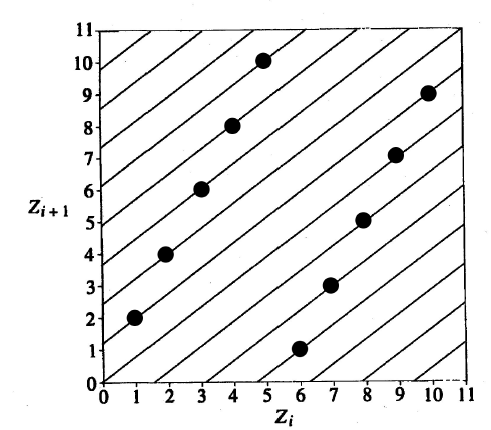
\includegraphics[width=0.5\textwidth]{img/14/korelacje.png}
        \label{fig:my_label}
    \end{figure}
\end{frame}
    \begin{frame}
	Kiedyś IBM wsławił się zdaniem: ``{\it gwarantuje tylko losowość każdej liczby indywidualnie }''
    \newline
    \newline
	b) {\it niższe bity są} ``{\it mniej losowe}'' niż {\it wyższe}:

    - nie wykorzystywać liczb losowych w {\it kawałkach},

	- np. do generowania liczb losowych $\in[1, 10 ]$

	używać:

	$J=1+INT(10.0*$RANF (iseed) $)$

	a nie:

	$J=1+MOD(INT(100000.0*RANF($iseed)$),\ 10)$
    \end{frame}
